% !TEX root = ../main.tex
\clearpage
\phantomsection
\section*{4 \textbf{Theoretical Framework}}
\label{sec:theoretical-framework}
\addcontentsline{toc}{section}{4 Theoretical Framework}

This study is grounded in hyperlink-citation theory, construct (domain) alignment, and computational complexity theory to compare EndorseRank against Adaptive Weighted PageRank (AWP) across three core constructs: Reputation Structure, Trading Success Alignment, and Computational Efficiency. Each construct links directly to the parameter definitions introduced earlier in the research objectives and expected-results framework and supports testable hypotheses.


\phantomsection
\subsection*{4.1 Constructs and Variable Mapping}
\label{sec:constructs-and-variable-mapping}
\addcontentsline{toc}{subsection}{4.1 Constructs and Variable Mapping}

Table~1 maps each evaluation construct to its variables and operational measures.

\begin{longtable}{>{\raggedright\arraybackslash}p{0.25\linewidth}>{\raggedright\arraybackslash}p{0.36\linewidth}>{\raggedright\arraybackslash}p{0.29\linewidth}}
\caption{Evaluation Constructs and Associated Variables}\\
\toprule
\textbf{Construct} & \textbf{Associated variables} & \textbf{Operational measures} \\
\midrule
Reputation Structure & EndorseRank score, AWP score, rank ordering, rank divergence & Spearman's rho, Kendall's tau, top-k overlap \\
\addlinespace
Trading Success Alignment & GMX close-success count, realized gain proxy, close success rate, reputation scores & Spearman's rho, Kendall's tau vs.\ each proxy \\
\addlinespace
Computational Efficiency & Graph build time, PageRank convergence time, memory usage, iteration count & Runtime, peak memory, iterations to tolerance \\
\addlinespace
\bottomrule
\end{longtable}

\phantomsection
\subsection*{4.2 Conceptual Model}
\label{sec:conceptual-model}
\addcontentsline{toc}{subsection}{4.2 Conceptual Model}

Figure~1 presents the conceptual model: the EndorseRank vs.\ AWP comparison is evaluated across three constructs (Reputation Structure, Trading Success Alignment, and Computational Efficiency), each with a corresponding testable hypothesis (H1--H3).


\begin{center}
% !TEX root = ../main.tex
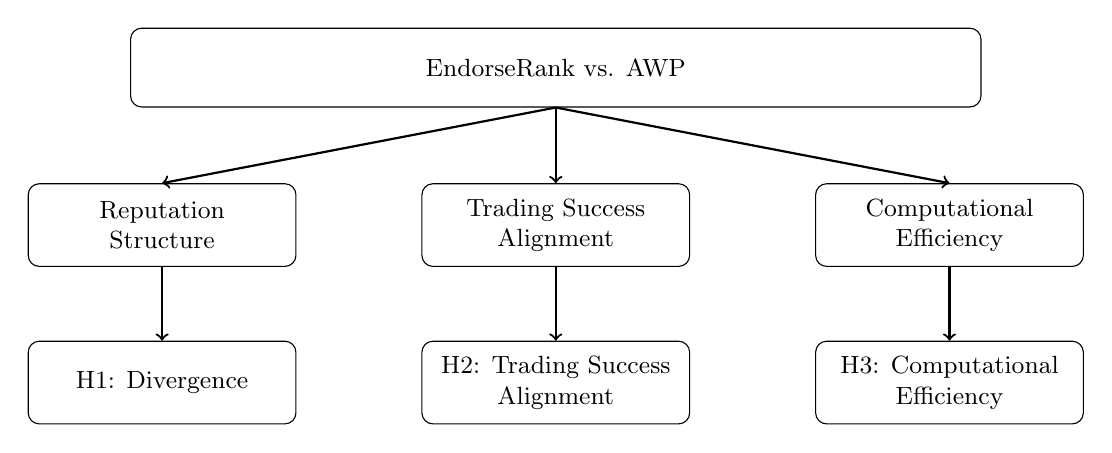
\begin{tikzpicture}[
  font=\small,
  box/.style={draw, rounded corners, align=center, minimum width=10.8cm, minimum height=1.0cm},
  smallbox/.style={draw, rounded corners, align=center, minimum width=3.4cm, minimum height=1.05cm},
  arrow/.style={->, thick}
]
\node[box] (center) at (0,2.6) {EndorseRank vs. AWP};

\node[smallbox] (rep) at (-5,0.6) {Reputation\\Structure};
\node[smallbox] (risk) at (0,0.6) {Trading Success\\Alignment};
\node[smallbox] (eff) at (5,0.6) {Computational\\Efficiency};

\node[smallbox] (h1) at (-5,-1.4) {H1: Divergence};
\node[smallbox] (h2) at (0,-1.4) {H2: Trading Success\\Alignment};
\node[smallbox] (h3) at (5,-1.4) {H3: Computational\\Efficiency};

\draw[arrow] (center.south) -- (rep.north);
\draw[arrow] (center.south) -- (risk.north);
\draw[arrow] (center.south) -- (eff.north);

\draw[arrow] (rep.south) -- (h1.north);
\draw[arrow] (risk.south) -- (h2.north);
\draw[arrow] (eff.south) -- (h3.north);
\end{tikzpicture}


\vspace{0.4em}
Figure 1: EndorseRank vs. AWP: hypotheses and evaluation constructs
\end{center}

\textbf{H1 (Divergence): }EndorseRank and AWP will yield significantly different wallet orderings, demonstrating that an approve/permit--based endorsement graph creates a distinct reputation structure.


\textbf{H2 (Trading Success Alignment): }EndorseRank's scores will correlate more strongly with GMX V2 trading-success proxies (close-success count and realized gain proxy) than AWP's scores, indicating superior domain-intuition alignment.


\textbf{H3 (Computational Efficiency): }EndorseRank will require less runtime, memory, and fewer iterations to converge than AWP, demonstrating practical scalability advantages.


\phantomsection
\subsection*{4.3 Theoretical Justification}
\label{sec:theoretical-justification}
\addcontentsline{toc}{subsection}{4.3 Theoretical Justification}

\textbf{Hyperlink--Citation Semantics: }The original PageRank algorithm (Page et al., 1998) evaluates a webpage's importance by the structure of inbound hyperlinks, treating each link as a citation and modeling a random surfer who follows links with a damping probability. Do et al.\ (2023) apply this propagation logic to Ethereum transaction graphs, weighting edges by transfer value and time-decay so that reputation flows along observed economic ties. This study extends the same citation-based propagation to ERC-20 approve/permit edges because allowances are explicit, on-chain delegations of spending authority (Ethereum Improvement Proposals, 2015; Ethereum Improvement Proposals, 2020). Unlike token transfers, which may reflect trading or automated routing without trust intent, an allowance records a durable authorization state until revoked. Graph-based risk models on Ethereum (Lin et al., 2024) further show that network structure carries risk-relevant information beyond raw activity counts, supporting the use of a directed endorsement graph rather than transfer volume alone.


\textbf{Domain Alignment Framework: }In measurement theory, construct alignment assesses how well an indicator tracks an observable outcome of interest (Cronbach \& Meehl, 1955). For rank-based reputation scoring, Spearman's rho and Kendall's tau are appropriate because they evaluate monotonic and pairwise ordering agreement between reputation scores and domain proxies without assuming a classification threshold (Do et al., 2023). Following Do et al.\ (2023), who validated PageRank against in-degree and in-value, we treat GMX V2 \textbf{close-success count} and \textbf{realized gain proxy} as observable trading-success measures on Arbitrum One. Reputation scores that align with these proxies therefore satisfy the study's domain-intuition requirement without claiming external ground-truth loan-repayment labels.


\textbf{Leveraged Exposure and Trading Success Alignment: }GMX V2 perpetual swap positions represent collateralized leveraged exposure: the trader posts margin and takes directional risk on an underlying asset through long or short positions. A profitable \textbf{PositionDecrease} close (positive \textbf{basePnlUsd}, excluding position liquidation) functionally resembles successfully managing borrowed or leveraged exposure---analogous to borrowing and fulfilling obligations in a credit context.


\textbf{Computational Complexity Theory: }PageRank's time complexity per iteration is $O(|E|)$ (Page et al., 1998). Approve/permit graphs are sparser than transfer-based graphs (fewer edges $|E|$), leading to lower per-iteration cost, faster convergence, and reduced memory usage.


\textbf{Scope and Future Extensions: }This proposal prioritizes interpretable graph propagation with verifiable on-chain signals over black-box predictive models. Supervised and representation-learning approaches to DeFi credit scoring (Ghosh et al., 2024; Kotb, 2023) can improve ranking performance but often sacrifice transparency and auditability under pseudonymity constraints emphasized by Packin and Lev-Aretz (2024). EndorseRank therefore stays within the PageRank family so that each score remains traceable to explicit allowance edges. Future work may combine endorsement-graph features with DeFi-informed representation learning, but such extensions are outside the present study's scope.


\phantomsection
\subsection*{4.4 Implications for Research Design}
\label{sec:implications-for-research-design}
\addcontentsline{toc}{subsection}{4.4 Implications for Research Design}

The research design applies the constructs above through the following measurement and analysis steps.

\textbf{Measurement: }Compute EndorseRank and AWP scores for a matched sample of GMX V2--active wallets on Arbitrum One, derive close-success count, realized gain proxy, and close success rate from \textbf{PositionDecrease} events over a defined observation window, and profile each algorithm's runtime, memory usage, and iterations to convergence.


Hypothesis testing and interpretation follow the measurement steps above and are organized as follows.


\proposalSubheading{Analysis:}

\textbf{H1 }via rank agreement between EndorseRank and AWP scores (Spearman's \emph{\(\rho\)}, Kendall's \emph{\(\tau\)}, top-\emph{k} overlap), testing whether these coefficients differ significantly from perfect concordance


\textbf{H2 }via rank correlation between reputation scores and GMX trading-success proxy rankings (Spearman's \emph{\(\rho\)}, Kendall's \emph{\(\tau\)}). Spearman's rho captures monotonic rank agreement; Kendall's tau measures pairwise ordering agreement. These metrics are justified because reputation scores and trading-success proxies are continuous rank variables rather than binary default labels, following the domain-alignment approach in Do et al.\ (2023).


\textbf{H3 }via paired benchmarks of runtime, peak memory, and iteration counts


\textbf{Contribution: }By anchoring our hypotheses in established theories, this framework ensures that empirical results will offer both scholarly rigor and practical relevance, demonstrating EndorseRank's advantages in producing a semantically meaningful, domain-aligned, and efficient on-chain reputation metric.
